\documentclass[12pt,a4paper]{article}
\usepackage[left=3cm, right=3cm, top=3cm]{geometry}

\usepackage{geometry}
\usepackage{graphicx}

\begin{document}
	\begin{center}
		\thispagestyle{empty}
		\vspace{3cm}
		\textbf{1st HOMEWORK\\
			Mathematical Modeling Q Class - KM184701\\}
		\vspace{0.75cm}
		\textbf{\large AUTOWASHER SPRING VIBRATIONS MODELING AND ITS SIMULATION}
		\vspace{2cm}
			
		
\includegraphics[width=175px]{picits.png}\\\vspace{3cm}
		\textbf{Lecturer :}\\Prof. Dr. Basuki Widodo, M.Sc\\
		\vspace{0.75cm}
		
		\textbf{Written by:}\\
		\begin{tabular}{ll}
			Venansius Ryan Tjahjono&06111540000043\\
			Titin Junik Ambarwati&06111540000065\\
			Vira Diana Ulnazilla&06111540000066\\
			Sumihar Christian N.S.&06111540000115
		\end{tabular}\\
		\vspace{2cm}	
		MATHEMATICS DEPARTMENT\\
		FACULTY OF MATHEMATICS, COMPUTATION, AND DATA SCIENCES\\
		INSTITUT TEKNOLOGI SEPULUH NOPEMBER\\
		SURABAYA\\
		2018
	\end{center}
	\pagebreak
	\begin{center}
		\Huge
		\textbf{Autowasher Spring Vibrations Problem}
	\end{center}
	Bias spring resonance problems encountered during the development of the suspension for the F and P electronic autowasher "Gentle Annie" $(1985)$. At $1100$ rpm when the washing machine was in spin mode the bias spring would vibrate wildly and make contact with the pulley.
	\begin{figure}[h]
		\begin{center}
			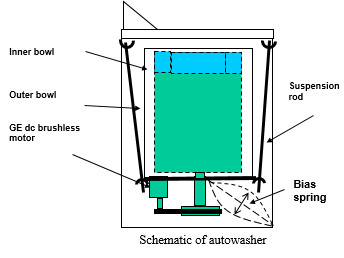
\includegraphics[width=400px]{wave0.PNG}
		\end{center}
	\end{figure}
	
\part{Modeling the Problem}

	The spring was long and slender like an elastic string. I recalled something I had learned in Engineering Mathematics II (The Predecessor of MM3):
	
	\textbf{How to derive the equation governing small transverse vibrations of an elastic string that is stretched to length L and then fixed at its endpoints.}
	\begin{figure}[h]
		\begin{center}
			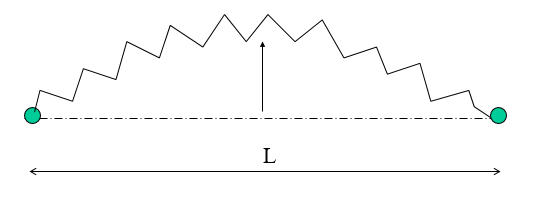
\includegraphics{wave1.PNG}
		\end{center}
	\end{figure}
	
	\textbf{Assumption}
	\begin{itemize}
		\item Mass per unit length is constant
		\item Gravity can be neglected
		\item Motion is in one plane
	\end{itemize}

	Modelling the spring as an elastic string. Consider a "free body diagram" of at string segment :
	\begin{figure}[h]
	\begin{center}
		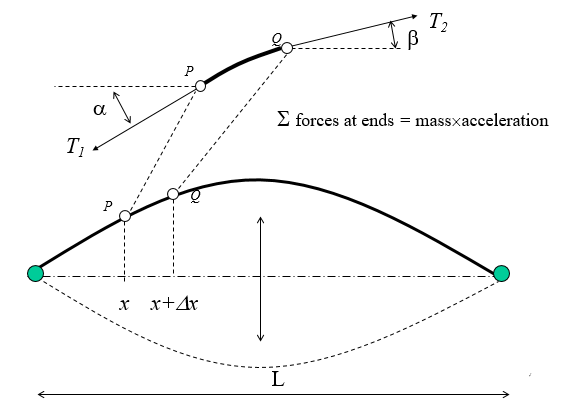
\includegraphics{wave2.PNG}
	\end{center}
	\end{figure}\\
	
	Now consider the forces acting on this string segment. we will find the deflection $u(x,t)$ at any point $x$ and $t>0$.
	\begin{figure}[h]
		\begin{center}
			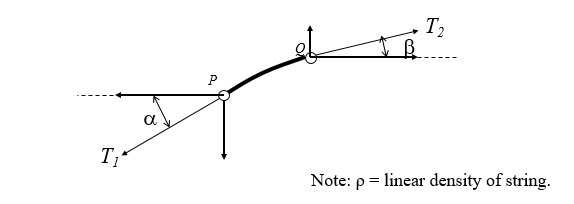
\includegraphics{wave3.PNG}
		\end{center}
	\end{figure}\\

	Horizontal Direction :
	\begin{equation}\label{}
	T_1 \cos \alpha \approx T_2 \cos \beta \approx T
	\end{equation}
	
	Vertical Direction :
	\begin{equation}\label{}
	T_2 \sin \beta - T_1 \sin \alpha = \rho \triangle x \frac{\partial{^2u}}{\partial{t^2}}  
	\end{equation}

	Divided equation $(2)$ by equation $(1)$ to get equation $(3)$ :
	
	$$\frac{T_2 \sin \beta}{T_2 \cos \beta}-\frac{T_1 \sin \alpha}{T_1 \cos \alpha} = \rho \frac{\triangle x}{T} \triangle x \frac{\partial{^2 u}}{\partial{t^2}}$$

	\begin{equation}\label{} \tan \beta - \tan \alpha = \rho \frac{\triangle x}{T} \triangle x \frac{\partial{^2 u}}{\partial{t^2}}
	\end{equation}
	
	Note:
	\begin{itemize}
	\item $\tan\alpha$ = string slope at $x $ and,\\
	\item $\tan \beta $= string slope at$ x + \triangle x$
	\end{itemize}

	\begin{figure}[h]
		\begin{center}
			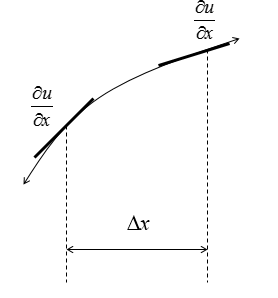
\includegraphics[width=200px]{wave4.PNG}
		\end{center}
	\end{figure}
	\pagebreak
	Thus
	$$\tan \beta = [\frac{\partial{u}} {\partial {x}}]_{x+\triangle x}$$
	and get equation $(4)$ :
	\begin{equation}\label{}
	\tan \beta = [\frac{\partial{u}} {\partial {x}}]_x
	\end{equation}
	
	After dividing equation $(3)$ by $T\triangle x $, and subtituing equation $(4)$ for the $\tan$ functions, we have :
	$$([\frac{\partial{u}}{\partial{x}}]_{x+\triangle x}-[\frac{\partial{u}} {\partial {x}}]_x)(\frac{1}{\triangle x}) = \frac {\rho}{T}\frac{\partial{^2 u}}{\partial{t^2}}$$
	
	Now let $\triangle x \to 0$\\
	$$\frac {[\frac{\partial{u}}{\partial{x}}]_{x+\triangle x}-[\frac{\partial{u}} {\partial {x}}]_x}{\triangle x} = \frac {\rho}{T}\frac{\partial{^2 u}}{\partial{t^2}}$$ 
	
	By letting $\triangle x \to 0$, we have obtained the one dimensional wave equation :
	$$\frac{\partial{^2 u}}{\partial{x^2}} = \frac {\rho}{T}\frac{\partial{^2 u}}{\partial{t^2}}$$
	
	Rearrange and set $c^2 = T/\rho$:
	\begin{equation}\label{}
	\frac{\partial{^2 u}}{\partial{t^2}} = c^2 \frac{\partial{^2 u}}{\partial{x^2}}
	\end{equation}\\
	
\part{The Solution to Obtained The Autowasher Spring}
	
	Instead of guessing we could start looking for a solution by making the assumption that it will be some function of $x$ multiplied by a function of $t$ :
	$$u(x,t) = X(x) T(t)$$
	
	We obtain the solution using the method of 
	\begin{center}
	\textbf{"Separation of Variables"}
	\end{center}

	Substitute the solution $u = X(x)T(t)$ into equation $(5)$:
	$$\frac{\partial{^2 u}}{\partial{t^2}} = c^2 \frac{\partial{^2 u}}{\partial{x^2}}$$
	You get :
	$$ X \frac{\partial{^2 T}}{\partial{t^2}} = c^2 \frac{\partial{^2 X}}{\partial{x^2}} T$$
	
	Now separate variables (get everything that's a function of $x$ on one side and everything that's a function of t on the other):
	$$\frac{\frac{\partial{^2 T}}{\partial{t^2}}}{c^2T} = \frac{\frac{\partial{^2 X}}{\partial{x^2}}}{X}$$
	
	Both sides are equal to a constant. Call it k:
	$$\frac{\frac{\partial{^2 T}}{\partial{t^2}}}{c^2T} = \frac{\frac{\partial{^2 X}}{\partial{x^2}}}{X} = k $$
	
	We get the two equations :\\
	Time $(t)$ only\\
	$$\frac{d^2T}{dt^2} - kc^2T = 0$$
	Distance $(x)$ only\\
	$$\frac{d^2X}{dx^2} - kX = 0$$
	
	Choose a sign for the constant that will give you sensible results.\\
	$k$ should be negative\\
	$k=-\lambda^2$\\
	you now get 2 differential equations :\\
	\begin{equation}\label{}
	{\frac{d^2T}{dt^2} - \lambda^2 c^2T = 0}\\
	{\frac{d^2X}{dx^2} - \lambda^2 X = 0}
	\end{equation}\\
	
	Solutions to $T$ and $X$ are:
	\begin{equation}\label{}
	{T = A \sin (\lambda c t) + B \cos (\lambda c t)}\\
	{X = C \sin (\lambda x) + D \cos (\lambda x)}
	\end{equation}\\
	
	The solution for u(x,t) equals X times T:
	\begin{equation}\label{}u(x,t) = (A sin (\lambda x)+ B \cos (\lambda x)(C \sin (c\lambda t)+ D \cos (c\lambda t)))
	\end{equation}
	
	Boundary Conditions :
	\begin{figure}[h]
		\begin{center}
			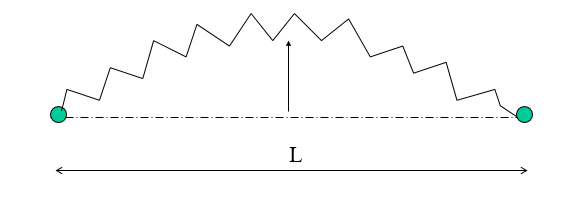
\includegraphics[width=400px]{wave5.PNG}
		\end{center}
	\end{figure}
	
	At t $x=0,  u(0,t)=0$\\
	$$u(0,t)=X(0)T(t)=B(C \sin (c\lambda t)+D \cos (c\lambda t)) = 0$$\\
	Thus $B = 0$\\
	At t $x=L,  u(l,t)=0$\\
	$$u(L,t)=X(L)T(t)=A \sin(\lambda L)(C \sin (c\lambda t)+D \cos (c\lambda t)) = 0$$\\
	So \\
	$\sin (\lambda L)=0$\\
	or $\lambda L = n \pi$, where $n = 0,1,2,3,. . .$\\
	So\\
	$$u_n(x,t) = A_n \sin \left(\frac{n\pi x}{L}\right)\left[C_n \sin\left(\frac{n\pi c t}{L}\right)+D_n \cos \left(\frac{n\pi c t}{L}\right)\right]$$\\
	or\\
	\begin{equation}\label{}
	u_n(x,t) = \sin\left(\frac{n\pi x}{L}\right)\left[a_n \sin\left(\frac{n\pi c t}{L}\right)+b_n\cos \left(\frac {n\pi c t}{L}\right)\right]
	\end{equation}
	$n = 1,2,3,. . .$ Note $n=0$ gives $u_0 = 0$
	
	\begin{center}
	\textbf{"$1^{st}$ Spring Mode"}
	\end{center}

	\begin{figure}[h]
	\begin{center}
		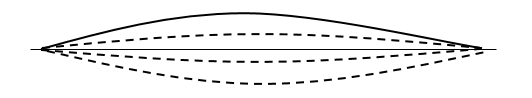
\includegraphics[width=400px]{wave6.PNG}
		$u_1(x,t)$
	\end{center}
	\end{figure}
	
	$$u_1(x,t) = \sin\left(\frac{\pi}{L}\right)\left[a_1 \sin\left(\frac{\pi c t}{L}\right)+b_1\cos \left(\frac {\pi c t}{L}\right)\right]$$
	
	\part{MATLAB Simulation}
\end{document}